


\begin{transitionframe}{Images/Transitions/RioChrist3}{black}
\textbf{Proof Overview}
\end{transitionframe}


\newcommand{\phantomCOne}{
\begin{prooftree}
\AXC{$\phantom{\textbf{A3}}$} \noLine
\UIC{$\phantom{P(G)}$}
		\AXC{$\phantom{\textbf{A2}}$} \noLine
		\UIC{$\phantom{\all \varphi. \all \psi.[(P(\varphi) \wedge \nec \all x.[\varphi(x) \imp \psi(x)]) \imp P(\psi)]}$}
					\AXC{$\phantom{\textbf{A1a}}$} \noLine
					\UIC{$\phantom{\all \varphi. [P(\neg \varphi) \imp \neg P(\varphi)]}$} \noLine
				\BIC{$\phantom{\textbf{T1: } \all \varphi. [P(\varphi) \imp \pos \ex x.\varphi(x)]}$} \noLine
	\BIC{$\phantom{\textbf{C1: } \pos \ex z. G(z)}$}
\end{prooftree}
}

\newcommand{\phantomTTwo}{
\begin{prooftree}
						\AXC{$\phantom{\textbf{A1b}}$} \noLine
						\UIC{$\phantom{\all \varphi. [\neg P(\varphi) \imp P(\neg \varphi)]}$}
								\AXC{$\phantom{\textbf{A4}}$} \noLine
								\UIC{$\phantom{ \all \varphi.[P(\varphi) \to \Box \; P(\varphi)]} $} \noLine
							\BIC{$\phantom{\textbf{T2: } \all y.[G(y) \imp \ess{G}{y}]}$}
									\AXC{$\phantom{\textbf{A5}}$} \noLine
									\UIC{$ \phantom{P(E)} $} \noLine
								\BIC{$\phantom{\textbf{L1: } \ex z. G(z) \imp \nec \ex x. G(x)}$} \noLine
								\UIC{$\phantom{\pos \ex z. G(z) \imp \pos \nec \ex x. G(x)}$}
										\AXC{$\phantom{\textbf{S5}}$} \noLine
 										\UIC{$\phantom{\all \xi.[\pos \nec \xi \imp \nec \xi]}$} \noLine	
									\BIC{$\phantom{\textbf{L2: } \pos \ex z. G(z) \imp \nec \ex x. G(x)}$}
\end{prooftree}
}

\newcommand{\phantomDOne}{
$$
\phantom{
\textbf{D1: } G(x) \equiv \forall \varphi. [P(\varphi) \to \varphi(x)]}
$$
}

\newcommand{\DOne}{
$$
\textbf{D1: } G(x) \equiv \forall \varphi. [P(\varphi) \to \varphi(x)]
$$
}

\newcommand{\phantomDTwo}{
$$
\phantom{
\textbf{D2: } \ess{\varphi}{x} \equiv \varphi(x) \wedge \all \psi. (\psi(x) \imp \nec \all x. (\varphi(x) \imp \psi(x)))
}
$$
}

\newcommand{\DTwo}{
$$
\textbf{D2: } \ess{\varphi}{x} \equiv \textcolor{blue}{\varphi(x)} \wedge \all \psi. (\psi(x) \imp \nec \all x. (\varphi(x) \imp \psi(x)))
$$
}


\newcommand{\phantomDThree}{
$$
\phantom{
\textbf{D3: } E(x) \equiv \all \varphi.[\ess{\varphi}{x} \imp \nec \ex y.\varphi(y)]
}
$$
}

\newcommand{\DThree}{
$$
\textbf{D3: } E(x) \equiv \all \varphi.[\ess{\varphi}{x} \imp \nec \ex y.\varphi(y)]
$$
}


\begin{frame}[shrink]{Proof Overview}

\phantomDOne

\phantomDTwo

\phantomDThree

\phantomCOne

\phantomTTwo

\begin{prooftree}
\AXC{$\phantom{\textbf{C1: } \pos \ex z. G(z)}$}
		\AXC{$\phantom{\textbf{L2: } \pos \ex z. G(z) \imp \nec \ex x. G(x)}$} \noLine
	\BIC{$\textbf{T3: } \nec \ex x. G(x) $}
\end{prooftree}

\end{frame}




\begin{frame}[shrink]{Proof Overview}

\phantomDOne

\phantomDTwo

\phantomDThree

\phantomCOne

\phantomTTwo

\begin{prooftree}
\AXC{$\textbf{C1: } \pos \ex z. G(z)$}
		\AXC{$\phantom{\textbf{L2: } \pos \ex z. G(z) \imp \nec \ex x. G(x)}$}
	\BIC{$\textbf{T3: } \nec \ex x. G(x) $}
\end{prooftree}

\end{frame}

\newcommand{\TThree}{
\begin{prooftree}
\AXC{$\textbf{C1: } \pos \ex z. G(z)$}
		\AXC{$\textbf{L2: } \pos \ex z. G(z) \imp \nec \ex x. G(x)$}
	\BIC{$\textbf{T3: } \nec \ex x. G(x) $}
\end{prooftree}	
}


\begin{frame}[shrink]{Proof Overview}

\phantomDOne

\phantomDTwo

\phantomDThree

\phantomCOne

\phantomTTwo

\TThree

\end{frame}

\begin{frame}[shrink]{Proof Overview}

\phantomDOne

\phantomDTwo

\phantomDThree

\phantomCOne

\begin{prooftree}
						\AXC{$\phantom{\textbf{A1b}}$} \noLine
						\UIC{$\phantom{\all \varphi. [\neg P(\varphi) \imp P(\neg \varphi)]}$}
								\AXC{$\phantom{\textbf{A4}}$} \noLine
								\UIC{$\phantom{ \all \varphi.[P(\varphi) \to \Box \; P(\varphi)]} $} \noLine
							\BIC{$\phantom{\textbf{T2: } \all y.[G(y) \imp \ess{G}{y}]}$}
									\AXC{$\phantom{\textbf{A5}}$} \noLine
									\UIC{$ \phantom{P(E)} $} \noLine
								\BIC{$\phantom{\textbf{L1: } \ex z. G(z) \imp \nec \ex x. G(x)}$} \noLine
								\UIC{$\phantom{\pos \ex z. G(z) \imp \pos \nec \ex x. G(x)}$}
										\AXC{$\phantom{\textbf{S5}}$} \noLine
 										\UIC{$\phantom{\all \xi.[\pos \nec \xi \imp \nec \xi]}$} \noLine	
									\BIC{$\textbf{L2: } \pos \ex z. G(z) \imp \nec \ex x. G(x)$}
\end{prooftree}

\TThree

\end{frame}


\begin{frame}[shrink]{Proof Overview}

\phantomDOne

\phantomDTwo

\phantomDThree

\phantomCOne

\begin{prooftree}
						\AXC{$\phantom{\textbf{A1b}}$} \noLine
						\UIC{$\phantom{\all \varphi. [\neg P(\varphi) \imp P(\neg \varphi)]}$}
								\AXC{$\phantom{\textbf{A4}}$} \noLine
								\UIC{$\phantom{ \all \varphi.[P(\varphi) \to \Box \; P(\varphi)]} $} \noLine
							\BIC{$\phantom{\textbf{T2: } \all y.[G(y) \imp \ess{G}{y}]}$}
									\AXC{$\phantom{\textbf{A5}}$} \noLine
									\UIC{$ \phantom{P(E)} $} \noLine
								\BIC{$\phantom{\textbf{L1: } \ex z. G(z) \imp \nec \ex x. G(x)}$} \noLine
								\UIC{$\phantom{\pos \ex z. G(z) \imp \pos \nec \ex x. G(x)}$}
										\AXC{$\textbf{S5}$} \dashedLine
 										\UIC{$\all \xi.[\pos \nec \xi \imp \nec \xi]$} 	
									\BIC{$\textbf{L2: } \pos \ex z. G(z) \imp \nec \ex x. G(x)$}
\end{prooftree}

\TThree

\end{frame}




\begin{frame}[shrink]{Proof Overview}

\phantomDOne

\phantomDTwo

\phantomDThree

\phantomCOne

\begin{prooftree}
						\AXC{$\phantom{\textbf{A1b}}$} \noLine
						\UIC{$\phantom{\all \varphi. [\neg P(\varphi) \imp P(\neg \varphi)]}$}
								\AXC{$\phantom{\textbf{A4}}$} \noLine
								\UIC{$\phantom{ \all \varphi.[P(\varphi) \to \Box \; P(\varphi)]} $} \noLine
							\BIC{$\phantom{\textbf{T2: } \all y.[G(y) \imp \ess{G}{y}]}$}
									\AXC{$\phantom{\textbf{A5}}$} \noLine
									\UIC{$ \phantom{P(E)} $} \noLine
								\BIC{$\phantom{\textbf{L1: } \ex z. G(z) \imp \nec \ex x. G(x)}$} \noLine
								\UIC{$\pos \ex z. G(z) \imp \pos \nec \ex x. G(x)$}
										\AXC{$\textbf{S5}$} \dashedLine
 										\UIC{$\all \xi.[\pos \nec \xi \imp \nec \xi]$} 	
									\BIC{$\textbf{L2: } \pos \ex z. G(z) \imp \nec \ex x. G(x)$}
\end{prooftree}

\TThree

\end{frame}




\begin{frame}[shrink]{Proof Overview}

\phantomDOne

\phantomDTwo

\phantomDThree

\phantomCOne

\begin{prooftree}
						\AXC{$\phantom{\textbf{A1b}}$} \noLine
						\UIC{$\phantom{\all \varphi. [\neg P(\varphi) \imp P(\neg \varphi)]}$}
								\AXC{$\phantom{\textbf{A4}}$} \noLine
								\UIC{$\phantom{ \all \varphi.[P(\varphi) \to \Box \; P(\varphi)]} $} \noLine
							\BIC{$\phantom{\textbf{T2: } \all y.[G(y) \imp \ess{G}{y}]}$}
									\AXC{$\phantom{\textbf{A5}}$} \noLine
									\UIC{$ \phantom{P(E)} $} \noLine
								\BIC{$\textbf{L1: } \ex z. G(z) \imp \nec \ex x. G(x)$} 
								\UIC{$\pos \ex z. G(z) \imp \pos \nec \ex x. G(x)$}
										\AXC{$\textbf{S5}$} \dashedLine
 										\UIC{$\all \xi.[\pos \nec \xi \imp \nec \xi]$} 	
									\BIC{$\textbf{L2: } \pos \ex z. G(z) \imp \nec \ex x. G(x)$}
\end{prooftree}

\TThree

\end{frame}



\begin{frame}[shrink]{Proof Overview}

\DOne

\phantomDTwo

\phantomDThree

\phantomCOne

\begin{prooftree}
						\AXC{$\phantom{\textbf{A1b}}$} \noLine
						\UIC{$\phantom{\all \varphi. [\neg P(\varphi) \imp P(\neg \varphi)]}$}
								\AXC{$\phantom{\textbf{A4}}$} \noLine
								\UIC{$\phantom{ \all \varphi.[P(\varphi) \to \Box \; P(\varphi)]} $} \noLine
							\BIC{$\phantom{\textbf{T2: } \all y.[G(y) \imp \ess{G}{y}]}$}
									\AXC{$\phantom{\textbf{A5}}$} \noLine
									\UIC{$ \phantom{P(E)} $} \noLine
								\BIC{$\textbf{L1: } \ex z. G(z) \imp \nec \ex x. G(x)$} 
								\UIC{$\pos \ex z. G(z) \imp \pos \nec \ex x. G(x)$}
										\AXC{$\textbf{S5}$} \dashedLine
 										\UIC{$\all \xi.[\pos \nec \xi \imp \nec \xi]$} 	
									\BIC{$\textbf{L2: } \pos \ex z. G(z) \imp \nec \ex x. G(x)$}
\end{prooftree}

\TThree

\end{frame}


\begin{frame}[shrink]{Proof Overview}

\DOne

\phantomDTwo

\qquad
\alert{$\textbf{D3*: } E(x) \equiv \nec \ex y. G(y)$} \only<2>{(cheating!)}

\phantomCOne

\begin{prooftree}
						\AXC{$\phantom{\textbf{A1b}}$} \noLine
						\UIC{$\phantom{\all \varphi. [\neg P(\varphi) \imp P(\neg \varphi)]}$}
								\AXC{$\phantom{\textbf{A4}}$} \noLine
								\UIC{$\phantom{ \all \varphi.[P(\varphi) \to \Box \; P(\varphi)]} $} \noLine
							\BIC{$\phantom{\textbf{T2: } \all y.[G(y) \imp \ess{G}{y}]}$}
									\AXC{$\phantom{\textbf{A5}}$} \noLine
									\UIC{$ P(E) $}
								\BIC{$\textbf{L1: } \ex z. G(z) \imp \nec \ex x. G(x)$} 
								\UIC{$\pos \ex z. G(z) \imp \pos \nec \ex x. G(x)$}
										\AXC{$\textbf{S5}$} \dashedLine
 										\UIC{$\all \xi.[\pos \nec \xi \imp \nec \xi]$} 	
									\BIC{$\textbf{L2: } \pos \ex z. G(z) \imp \nec \ex x. G(x)$}
\end{prooftree}

\TThree

\end{frame}


\begin{frame}[shrink]{Proof Overview}

\DOne

\phantomDTwo

\qquad
\alert{$\textbf{D3*: } E(x) \equiv \nec \ex y. G(y)$}
\qquad\qquad
$\textbf{D3: } E(x) \equiv \all \varphi.[\ess{\varphi}{x} \imp \nec \ex y.\varphi(y)]$
\phantomCOne

\begin{prooftree}
						\AXC{$\phantom{\textbf{A1b}}$} \noLine
						\UIC{$\phantom{\all \varphi. [\neg P(\varphi) \imp P(\neg \varphi)]}$}
								\AXC{$\phantom{\textbf{A4}}$} \noLine
								\UIC{$\phantom{ \all \varphi.[P(\varphi) \to \Box \; P(\varphi)]} $} \noLine
							\BIC{$\textbf{T2: } \all y.[G(y) \imp \ess{G}{y}]$}
									\AXC{$\phantom{\textbf{A5}}$} \noLine
									\UIC{$ P(E) $}
								\BIC{$\textbf{L1: } \ex z. G(z) \imp \nec \ex x. G(x)$} 
								\UIC{$\pos \ex z. G(z) \imp \pos \nec \ex x. G(x)$}
										\AXC{$\textbf{S5}$} \dashedLine
 										\UIC{$\all \xi.[\pos \nec \xi \imp \nec \xi]$} 	
									\BIC{$\textbf{L2: } \pos \ex z. G(z) \imp \nec \ex x. G(x)$}
\end{prooftree}

\TThree

\end{frame}


\begin{frame}[shrink]{Proof Overview}

\DOne

\phantomDTwo

\qquad
\alert{$\textbf{D3*: } E(x) \equiv \nec \ex y. G(y)$}
\qquad\qquad
$\textbf{D3: } E(x) \equiv \all \varphi.[\ess{\varphi}{x} \imp \nec \ex y.\varphi(y)]$
\phantomCOne

\begin{prooftree}
						\AXC{$\phantom{\textbf{A1b}}$} \noLine
						\UIC{$\phantom{\all \varphi. [\neg P(\varphi) \imp P(\neg \varphi)]}$}
								\AXC{$\phantom{\textbf{A4}}$} \noLine
								\UIC{$\phantom{ \all \varphi.[P(\varphi) \to \Box \; P(\varphi)]} $} \noLine
							\BIC{$\textbf{T2: } \all y.[G(y) \imp \ess{G}{y}]$}
									\AXC{$\textbf{A5}$} \dashedLine
									\UIC{$ P(E) $}
								\BIC{$\textbf{L1: } \ex z. G(z) \imp \nec \ex x. G(x)$} 
								\UIC{$\pos \ex z. G(z) \imp \pos \nec \ex x. G(x)$}
										\AXC{$\textbf{S5}$} \dashedLine
 										\UIC{$\all \xi.[\pos \nec \xi \imp \nec \xi]$} 	
									\BIC{$\textbf{L2: } \pos \ex z. G(z) \imp \nec \ex x. G(x)$}
\end{prooftree}

\TThree

\end{frame}



\begin{frame}[shrink]{Proof Overview}

\DOne

\phantomDTwo

\qquad
\alert{$\textbf{D3*: } E(x) \equiv \nec \ex y. G(y)$}
\qquad\qquad
$\textbf{D3: } E(x) \equiv \all \varphi.[\ess{\varphi}{x} \imp \nec \ex y.\varphi(y)]$
\phantomCOne

\begin{prooftree}
						\AXC{$\phantom{\textbf{A1b}}$} \noLine
						\UIC{$\phantom{\all \varphi. [\neg P(\varphi) \imp P(\neg \varphi)]}$}
								\AXC{$\phantom{\textbf{A4}}$} \noLine
								\UIC{$\phantom{ \all \varphi.[P(\varphi) \to \Box \; P(\varphi)]} $} \noLine
							\BIC{$\textbf{T2: } \all y.[G(y) \imp \ess{G}{y}]$}
									\AXC{$\textbf{A5}$} \dashedLine
									\UIC{$ P(E) $}
								\BIC{$\textbf{L1: } \ex z. G(z) \imp \nec \ex x. G(x)$} 
								\UIC{$\pos \ex z. G(z) \imp \pos \nec \ex x. G(x)$}
										\AXC{$\textbf{S5}$} \dashedLine
 										\UIC{$\all \xi.[\pos \nec \xi \imp \nec \xi]$} 	
									\BIC{$\textbf{L2: } \pos \ex z. G(z) \imp \nec \ex x. G(x)$}
\end{prooftree}

\TThree

\end{frame}


\newcommand{\LTwo}{
\begin{prooftree}
						\AXC{$\textbf{A1b}$} \dashedLine
						\UIC{$\all \varphi. [\neg P(\varphi) \imp P(\neg \varphi)]$}
								\AXC{$\textbf{A4}$} \dashedLine
								\UIC{$ \all \varphi.[P(\varphi) \to \Box \; P(\varphi)] $} 
							\BIC{$\textbf{T2: } \all y.[G(y) \imp \ess{G}{y}]$}
									\AXC{$\textbf{A5}$} \dashedLine
									\UIC{$ P(E) $}
								\BIC{$\textbf{L1: } \ex z. G(z) \imp \nec \ex x. G(x)$} 
								\UIC{$\pos \ex z. G(z) \imp \pos \nec \ex x. G(x)$}
										\AXC{$\textbf{S5}$} \dashedLine
 										\UIC{$\all \xi.[\pos \nec \xi \imp \nec \xi]$} 	
									\BIC{$\textbf{L2: } \pos \ex z. G(z) \imp \nec \ex x. G(x)$}
\end{prooftree}
}


\begin{frame}[shrink]{Proof Overview}

\DOne

\DTwo

\qquad
\alert{$\textbf{D3*: } E(x) \equiv \nec \ex y. G(y)$}
\qquad\qquad
$\textbf{D3: } E(x) \equiv \all \varphi.[\ess{\varphi}{x} \imp \nec \ex y.\varphi(y)]$

\phantomCOne

\LTwo

\TThree

\end{frame}


\begin{frame}[shrink]{Proof Overview}

\DOne

\DTwo

\qquad
\alert{$\textbf{D3*: } E(x) \equiv \nec \ex y. G(y)$}
\qquad\qquad
$\textbf{D3: } E(x) \equiv \all \varphi.[\ess{\varphi}{x} \imp \nec \ex y.\varphi(y)]$

\begin{prooftree}
\AXC{$\phantom{\textbf{A3}}$} \noLine
\UIC{$\phantom{P(G)}$}
		\AXC{$\phantom{\textbf{A2}}$} \noLine
		\UIC{$\phantom{\all \varphi. \all \psi.[(P(\varphi) \wedge \nec \all x.[\varphi(x) \imp \psi(x)]) \imp P(\psi)]}$}
					\AXC{$\phantom{\textbf{A1a}}$} \noLine
					\UIC{$\phantom{\all \varphi. [P(\neg \varphi) \imp \neg P(\varphi)]}$} \noLine
				\BIC{$\phantom{\textbf{T1: } \all \varphi. [P(\varphi) \imp \pos \ex x.\varphi(x)]}$} \noLine
	\BIC{$\textbf{C1: } \pos \ex z. G(z)$}
\end{prooftree}

\LTwo

\TThree

\end{frame}


\begin{frame}[shrink]{Proof Overview}

\DOne

\DTwo

\qquad
\alert{$\textbf{D3*: } E(x) \equiv \nec \ex y. G(y)$}
\qquad\qquad
$\textbf{D3: } E(x) \equiv \all \varphi.[\ess{\varphi}{x} \imp \nec \ex y.\varphi(y)]$

\begin{prooftree}
\AXC{$\phantom{\textbf{A3}}$} \noLine
\UIC{$P(G)$}
		\AXC{$\phantom{\textbf{A2}}$} \noLine
		\UIC{$\phantom{\all \varphi. \all \psi.[(P(\varphi) \wedge \nec \all x.[\varphi(x) \imp \psi(x)]) \imp P(\psi)]}$}
					\AXC{$\phantom{\textbf{A1a}}$} \noLine
					\UIC{$\phantom{\all \varphi. [P(\neg \varphi) \imp \neg P(\varphi)]}$} \noLine
				\BIC{$\phantom{\textbf{T1: } \all \varphi. [P(\varphi) \imp \pos \ex x.\varphi(x)]}$} 
	\BIC{$\textbf{C1: } \pos \ex z. G(z)$}
\end{prooftree}

\LTwo

\TThree

\end{frame}


\begin{frame}[shrink]{Proof Overview}

\DOne

\DTwo

\qquad
\alert{$\textbf{D3*: } E(x) \equiv \nec \ex y. G(y)$}
\qquad\qquad
$\textbf{D3: } E(x) \equiv \all \varphi.[\ess{\varphi}{x} \imp \nec \ex y.\varphi(y)]$

\begin{prooftree}
\AXC{$\textbf{A3}$} \dashedLine
\UIC{$P(G)$}
		\AXC{$\phantom{\textbf{A2}}$} \noLine
		\UIC{$\phantom{\all \varphi. \all \psi.[(P(\varphi) \wedge \nec \all x.[\varphi(x) \imp \psi(x)]) \imp P(\psi)]}$}
					\AXC{$\phantom{\textbf{A1a}}$} \noLine
					\UIC{$\phantom{\all \varphi. [P(\neg \varphi) \imp \neg P(\varphi)]}$} \noLine
				\BIC{$\phantom{\textbf{T1: } \all \varphi. [P(\varphi) \imp \pos \ex x.\varphi(x)]}$} 
	\BIC{$\textbf{C1: } \pos \ex z. G(z)$}
\end{prooftree}

\LTwo

\TThree

\end{frame}



\begin{frame}[shrink]{Proof Overview}

\DOne

\DTwo

\qquad
\alert{$\textbf{D3*: } E(x) \equiv \nec \ex y. G(y)$}
\qquad\qquad
$\textbf{D3: } E(x) \equiv \all \varphi.[\ess{\varphi}{x} \imp \nec \ex y.\varphi(y)]$

\begin{prooftree}
\AXC{$\textbf{A3}$} \dashedLine
\UIC{$P(G)$}
		\AXC{$\phantom{\textbf{A2}}$} \noLine
		\UIC{$\phantom{\all \varphi. \all \psi.[(P(\varphi) \wedge \nec \all x.[\varphi(x) \imp \psi(x)]) \imp P(\psi)]}$}
					\AXC{$\phantom{\textbf{A1a}}$} \noLine
					\UIC{$\phantom{\all \varphi. [P(\neg \varphi) \imp \neg P(\varphi)]}$} \noLine
				\BIC{$\textbf{T1: } \all \varphi. [P(\varphi) \imp \pos \ex x.\varphi(x)]$} 
	\BIC{$\textbf{C1: } \pos \ex z. G(z)$}
\end{prooftree}

\LTwo

\TThree

\end{frame}



\begin{frame}[shrink]{Proof Overview}

\DOne

\DTwo

\qquad
\alert{$\textbf{D3*: } E(x) \equiv \nec \ex y. G(y)$}
\qquad\qquad
$\textbf{D3: } E(x) \equiv \all \varphi.[\ess{\varphi}{x} \imp \nec \ex y.\varphi(y)]$

\begin{prooftree}
\AXC{$\textbf{A3}$} \dashedLine
\UIC{$P(G)$}
		\AXC{$\textbf{A2}$} \dashedLine
		\UIC{$\all \varphi. \all \psi.[(P(\varphi) \wedge \nec \all x.[\varphi(x) \imp \psi(x)]) \imp P(\psi)]$}
					\AXC{$\textbf{A1a}$} \dashedLine
					\UIC{$\all \varphi. [P(\neg \varphi) \imp \neg P(\varphi)]$}
				\BIC{$\textbf{T1: } \all \varphi. [P(\varphi) \imp \pos \ex x.\varphi(x)]$} 
	\BIC{$\textbf{C1: } \pos \ex z. G(z)$}
\end{prooftree}

\LTwo

\TThree

\end{frame}



\begin{frame}[shrink]{Proof Overview}

$$
\textbf{D1: } G(x) \equiv \forall \varphi. [P(\varphi) \to \varphi(x)]
$$

$$
\textbf{D2: } \ess{\varphi}{x} \equiv \varphi(x) \wedge \all \psi. (\psi(x) \imp \nec \all x. (\varphi(x) \imp \psi(x)))
$$

$$
\textbf{D3: } NE(x) \equiv \all \varphi.[\ess{\varphi}{x} \imp \nec \ex y.\varphi(y)]
$$

\begin{prooftree}
\AXC{$\textbf{A3}$} \dashedLine
\UIC{$P(G)$}
		\AXC{$\textbf{A2}$} \dashedLine
		\UIC{$\all \varphi. \all \psi.[(P(\varphi) \wedge \nec \all x.[\varphi(x) \imp \psi(x)]) \imp P(\psi)]$}
					\AXC{$\textbf{A1a}$} \dashedLine
					\UIC{$\all \varphi. [P(\neg \varphi) \imp \neg P(\varphi)]$} \doubleLine
				\BIC{$\textbf{T1: } \all \varphi. [P(\varphi) \imp \pos \ex x.\varphi(x)]$} \doubleLine
	\BIC{$\textbf{C1: } \pos \ex z. G(z)$}
\end{prooftree}





\begin{prooftree}
						\AXC{$\textbf{A1b}$} \dashedLine
						\UIC{$\all \varphi. [\neg P(\varphi) \imp P(\neg \varphi)]$}
								\AXC{$\textbf{A4}$} \dashedLine
								\UIC{$ \all \varphi.[P(\varphi) \to \Box \; P(\varphi)] $} \doubleLine
							\BIC{$\textbf{T2: } \all y.[G(y) \imp \ess{G}{y}]$}
									\AXC{$\textbf{A5}$} \dashedLine
									\UIC{$ P(NE) $} \doubleLine
								\BIC{$\textbf{L1: } \ex z. G(z) \imp \nec \ex x. G(x)$} \doubleLine
								\UIC{$\pos \ex z. G(z) \imp \pos \nec \ex x. G(x)$}
										\AXC{$\textbf{S5}$} \dashedLine
 										\UIC{$ \all \xi.[\pos \nec \xi \imp \nec \xi]$} \doubleLine	
									\BIC{$\textbf{L2: } \pos \ex z. G(z) \imp \nec \ex x. G(x)$}
\end{prooftree}

\begin{prooftree}
\AXC{$\textbf{C1: } \pos \ex z. G(z)$}
		\AXC{$\textbf{L2: } \pos \ex z. G(z) \imp \nec \ex x. G(x)$} \doubleLine
	\BIC{$\textbf{T3: } \nec \ex x. G(x) $}
\end{prooftree}

\end{frame}


% \begin{frame}{Scott's Version of G\"odel's Axioms, Definitions and Theorems}
% \begin{changemargin}{-0.9cm}{-0.8cm}
% \colorbox{black}{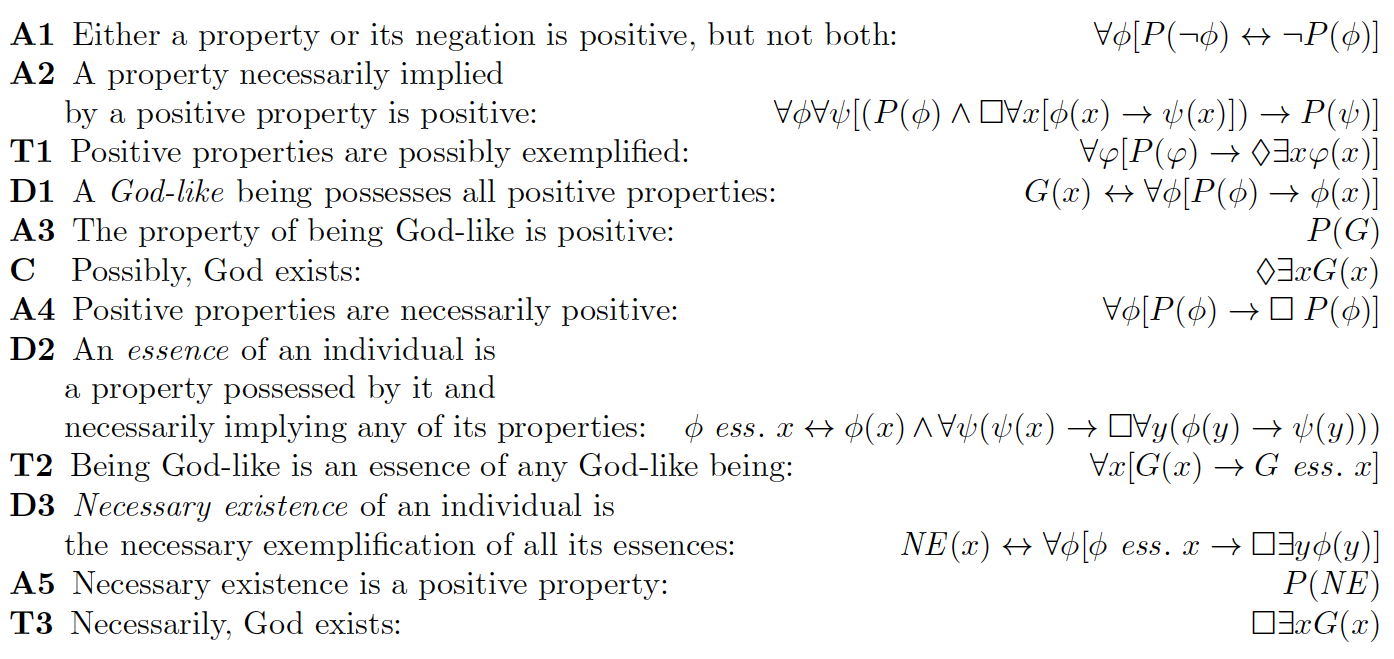
\includegraphics[width=12.4cm]{Images/ScottsScriptGrab.png}}
% \end{changemargin}
% \end{frame}



\begin{transitionframe}{Images/Transitions/ReligiousSymbols(Sowlos)(CC-BY-SA).png}{white}
\textbf{Modal Natural Deduction Proof}
\end{transitionframe}



\begin{frame}[shrink]{Natural Deduction Calculus}

\begin{unnamedCalculus}

\vspace{1em}

\s\s
\infer[\vee_E]{C}{A \vee B & \infer*{C}{\infer{A}{}} & \infer*{C}{\infer{B}{}}}
\s\s
\infer[\wedge_I]{A \wedge B}{A & B}
\s\s
\infer[\imp_I^n]{A \imp B}{ \infer*{B}{\infer[n]{A}{}} }

\vspace{2em}

\s\s
\infer[\vee_{I_1}]{A \vee B}{A}
\s\s
\infer[\wedge_{E_1}]{A}{A \wedge B}
\s\s
\infer[\imp_I]{A \imp B}{ B }

\vspace{2em}

\s\s
\infer[\vee_{I_2}]{A \vee B}{B}
\s\s
\infer[\wedge_{E_2}]{B}{A \wedge B}
\s\s
\infer[\imp_E]{B}{A & A \imp B}

\vspace{2em}

\s
\infer[\all_I]{\all x. A[x]}{ A[\alpha] }
\s
\infer[\all_E]{A[t]}{ \all x. A[x] }
\s\s
\infer[\ex_I]{\ex x. A[x]}{ A[t] }
\s
\infer[\ex_E]{A[\beta]}{ \ex x. A[x] }

\vspace{1em}

\s\s\s\s
$\neg A \equiv A \imp \bot$ 
\s\s\s 
\alert{\infer[\neg\neg_E]{A}{\neg\neg A}}

\vspace{1em}

\end{unnamedCalculus}

\end{frame}



\begin{frame}[shrink]{Natural Deduction Calculus}{Rules for Modalities}

\begin{unnamedCalculus}

\vspace{1em}

\s\s\s\s
\infer[\nec_I]{\nec A}{\alpha: \fbox{\infer*{A}{}} }
\s\s\s\s\s
\infer[\nec_E]{t: \fbox{ \infer*{}{A} }  }{\nec A}

\vspace{2em}

\pause

\alert{$$\pos A \equiv \neg \nec \neg A$$}

\pause

\vspace{2em}

\s\s\s\s
\infer[\pos_I]{\pos A}{t: \fbox{\infer*{A}{}} }
\s\s\s\s\s
\infer[\pos_E]{\beta: \fbox{ \infer*{}{A} }  }{\pos A}


\vspace{1em}

\end{unnamedCalculus}

\end{frame}


% \begin{frame}[shrink]{Natural Deduction Calculus}{Three tiny examples}

% \vspace{1em}

% \infer[\imp_I]{A \imp A}{\infer[n]{A}{}}


% \infer[\imp_I]{A \imp A}{\infer[n]{A}{}}


% \vspace{1em}

% \end{frame}


\begin{frame}{Natural Deduction Proofs}{T1 and C1}
\begin{prooftree}
        \AXC{\textbf{A2}} \dashedLine
        \UIC{$ \all \varphi. \all \psi.[(P(\varphi) \wedge \nec \all x.[\varphi(x) \imp \psi(x)]) \imp P(\psi)]$} \RightLabel{$\all_E$}
        \UIC{$ \all \psi.[(P(\rho) \wedge \nec \all x.[\rho(x) \imp \psi(x)]) \imp P(\psi)]$} \RightLabel{$\all_E$}
        \UIC{$(P(\rho) \wedge \nec \all x.[\rho(x) \imp \neg \rho(x)]) \imp P(\neg \rho)$} \doubleLine
        \UIC{$(P(\rho) \wedge \nec \all x.[\neg \rho(x)]) \imp P(\neg \rho)$}
                        \AXC{\textbf{A1a}} \dashedLine
                        \UIC{$\all \varphi.[ P(\neg \varphi) \imp \neg P(\varphi) ]$} \RightLabel{$\all_E$}
                        \UIC{$ P(\neg \rho) \imp \neg P(\rho) $} \doubleLine
                 \BIC{$ (P(\rho) \wedge \nec \all x.[\neg \rho(x)]) \imp \neg P(\rho) $} \doubleLine
                 \UIC{$ P(\rho) \imp \pos \ex x.\rho(x) $} \RightLabel{$\all_I$}
                 \UIC{\textbf{T1: }$\all \varphi.[ P(\varphi) \imp \pos \ex x.\varphi(x) ] $}
\end{prooftree}

\begin{prooftree}
\AXC{\textbf{A3}} \dashedLine
\UIC{$P(G)$}
                 \AXC{\textbf{T1}} \dashedLine
                 \UIC{$\all \varphi.[ P(\varphi) \imp \pos \ex x.\varphi(x) ]$} \RightLabel{$\all_E $}
                 \UIC{$ P(G) \imp \pos \ex x.G(x) $} \RightLabel{$\imp_E$}
    \BIC{$\pos \ex x. G(x)$}
\end{prooftree}
\end{frame}



\begin{frame}{Natural Deduction Proofs}{T2 (Partial)}
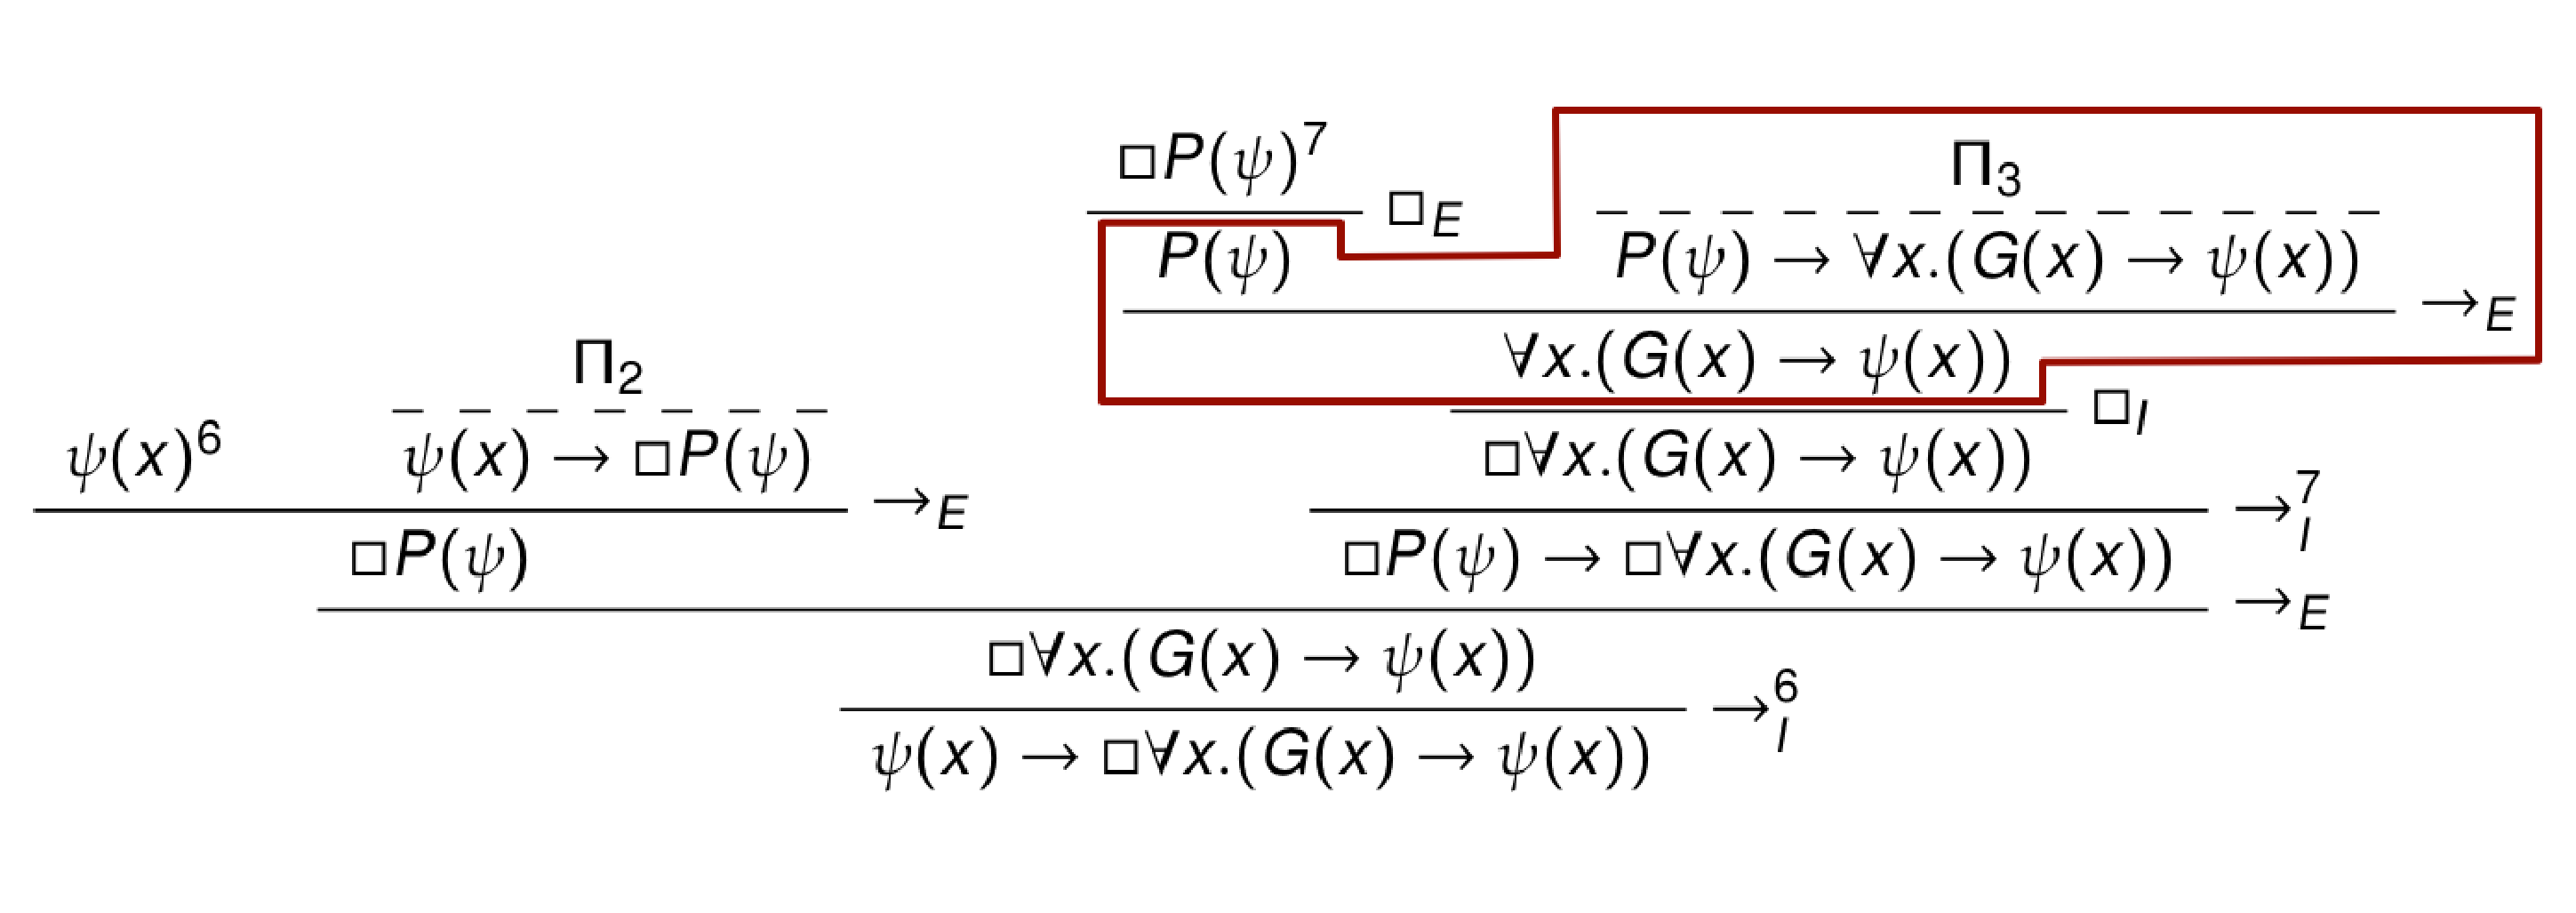
\includegraphics[scale=0.22]{Images/ProofOfT2Boxed.pdf}
\end{frame}
